\documentclass[a4paper, 11pt]{article}
\usepackage{comment} % enables the use of multi-line comments (\ifx \fi) 
\usepackage{lipsum} %This package just generates Lorem Ipsum filler text. 
\usepackage{fullpage} % changes the margin
\usepackage{graphicx}
\graphicspath{ {.} }
\begin{document}
%Header-Make sure you update this information!!!!
\noindent
\large\textbf{Lab Report} \hfill \textbf{Ivan Jurin} \\

\section*{Izvod}
Sustav raspolaze s $m$ pravila:\\

Ako $x$ je $A_{1}$ i $y$ je $B_{1}$ tada $z_{1}=p_{1}x+q_{1}y+r_{1}$\\

Ako $x$ je $A_{2}$ i $y$ je $B_{2}$ tada $z_{2}=p_{2}x+q_{2}y+r_{2}$\\

...\\

Ako $x$ je $A_{m}$ i $y$ je $B_{m}$ tada $z_{m}=p_{m}x+q_{m}y+r_{m}$\\
\\
Prijenosna funkcija koju sustav koristi definirane su izrazima:
$$\mu_{A_{i}}(x)=\frac{1}{1+e^{b_{i}(x-a_{i})}}$$
$$\mu_{B_{i}}(x)=\frac{1}{1+e^{c_{i}(y-d_{i})}}$$
Opcenito greska je definirana izrazom:
$$E_{k}=\frac{1}{2}(y_{k}-o_{k})^{2}$$
Azuriranje parametra gradijentnim spustom:
$$\psi(t+1) = \psi(t)-\eta\frac{\delta E_{k}}{\delta\psi}$$
Cilj je utvrditi parcijalne derivacije po svim parametrima $a_{i},b_{i},c_{i},d_{i},p_{i},q_{i},r_{i}$\\
Izvod pravila za azuriranje parametara $z_{i}$:\\
Izlaz sustava neizrazitog upravljanja definiran je kao tezinska suma:
$$o = \frac{\sum_{j=1}^{m}\gamma_{j}z_{j}}{\sum_{j=1}^{m}\gamma_{j}}$$
Pri cemu je jakost paljenja $i$-tog pravila i u promatranom slucaju ona je jednaka 
$$\gamma _{i} := T(A_{i}(x),B_{i}(x)) = A_{i}(x)B_{i}(x)$$ te su definirani 
$$\alpha_{i} := A_{i}(x),\beta_{i} := B_{i}(x) \rightarrow \gamma_{i} = \alpha_{i}\beta_{i}$$
Za potrebe izracuna parcijalne derivacije funkcije pogreske po parametrima $p_{i}$, $q_{i}$ i $r_{i}$ posluziti cemo se pravilom ulancavanja:
$$\frac{\partial E_{k}}{\partial p_{i}}=\frac{\partial E_{k}}{\partial o_{k}}\frac{\partial o_{k}}{\partial z_{i}}\frac{\partial z_{i}}{\partial p_{i}}$$
$$\frac{\partial E_{k}}{\partial q_{i}}=\frac{\partial E_{k}}{\partial o_{k}}\frac{\partial o_{k}}{\partial z_{i}}\frac{\partial z_{i}}{\partial q_{i}}$$
$$\frac{\partial E_{k}}{\partial r_{i}}=\frac{\partial E_{k}}{\partial o_{k}}\frac{\partial o_{k}}{\partial z_{i}}\frac{\partial z_{i}}{\partial r_{i}}$$
Pri cemu su:
\newcommand{\minusdEkdok}{(y_{k}-o_{k})}
$$\frac{\delta E_{k}}{\partial o_{k}} = \frac{\partial}{\partial o_{k}}\left (\frac{1}{2}(y_{k}-o_{k})^{2}\right )=-\minusdEkdok$$
\newcommand{\dokdzi}{\frac{\gamma_{i}}{\sum_{j=1}^{m}\gamma_{j}}}
\newcommand{\outfunc}{p_{i}x+q_{i}y+r_{i}}
$$\frac{\partial o_{k}}{\partial z_{i}} = \frac{\partial}{\partial z_{j}}\left (\frac{\sum_{j=1}^{m}\gamma_{j}z_{i}}{\sum_{j=1}^{m}\gamma_{j}}\right ) = \dokdzi$$
I:
$$\frac{\partial z_{i}}{\partial p_{i}} = \frac{\partial}{\partial p_{i}}(\outfunc) = x$$
$$\frac{\partial z_{i}}{\partial q_{i}} = \frac{\partial}{\partial q_{i}}(\outfunc) = y$$
$$\frac{\partial z_{i}}{\partial r_{i}} = \frac{\partial}{\partial r_{i}}(\outfunc) = 1$$
Pa su:
$$\frac{\partial E_{k}}{\partial p_{i}}=-\minusdEkdok\dokdzi x$$
$$\frac{\partial E_{k}}{\partial q_{i}}=-\minusdEkdok\dokdzi y$$
$$\frac{\partial E_{k}}{\partial r_{i}}=-\minusdEkdok\dokdzi$$
Za izvod ostalih parametara trebati ce nam slijedece derivacije:
\newcommand{\upperr}{\sum_{j=1}^{m}\gamma_{j}z_{j}}
\newcommand{\lowerr}{\sum_{j=1}^{m}\gamma_{j}}
$$\frac{\partial o_{k}}{\partial\gamma_{i}} = \frac{\partial}{\partial\gamma_{i}}\left (\frac{\upperr}{\lowerr}\right )=$$
$$= \frac{\frac{\partial}{\partial\gamma_{i}}\left (\upperr\right )\left(\lowerr\right)-\frac{\partial}{\partial\gamma_{i}}\left (\lowerr\right )\left(\upperr\right)}{\left(\lowerr\right)^{2}}$$
\newcommand{\dokdgamma}{ \frac{\sum_{j=1,j\neq i}^{m}\gamma_{j}(z_{i}-z_{j})}{\left(\lowerr\right)^{2}}}
\newcommand{\dgammadalpha}{ \beta_{i}}
\newcommand{\dgammadbeta}{\alpha_{i}}
$$=\dokdgamma$$
$$\frac{\partial \gamma_{i}}{\partial\alpha_{i}} = \frac{\partial}{\partial\alpha_{i}}\left(\alpha_{i}\beta_{i}\right)= \dgammadalpha$$
$$\frac{\partial \gamma_{i}}{\partial\beta_{i}} = \frac{\partial}{\partial\beta_{i}}\left(\alpha_{i}\beta_{i}\right)= \dgammadbeta$$
Izvod derivacija za parametre $a_{i}$ i $b_{i}$:
$$\frac{\partial E_{k}}{\partial a_{i}}=\frac{\partial E_{k}}{\partial o_{k}}\frac{\partial o_{k}}{\partial \gamma_{i}}\frac{\partial \gamma_{i}}{\partial \alpha_{i}}\frac{\partial \alpha_{i}}{\partial a_{i}}$$
$$\frac{\partial E_{k}}{\partial b_{i}}=\frac{\partial E_{k}}{\partial o_{k}}\frac{\partial o_{k}}{\partial \gamma_{i}}\frac{\partial \gamma_{i}}{\partial \alpha_{i}}\frac{\partial \alpha_{i}}{\partial b_{i}}$$
Potrebno je jos izracunati slijedece:
\newcommand{\sigmoidalphad}{\alpha_{i}(1-\alpha_{i})}
\newcommand{\dalphada}{\sigmoidalphad b_{i}}
\newcommand{\dalphadb}{\sigmoidalphad (a_{i}-x)}
\newcommand{\sigmoidbetad}{\beta_{i}(1-\beta_{i})}
\newcommand{\dbetadc}{\sigmoidbetad d_{i}}
\newcommand{\dbetadd}{\sigmoidbetad (c_{i}-y)}
$$\frac{\partial \alpha_{i}}{\partial a_{i}} = \dalphada$$
$$\frac{\partial \alpha_{i}}{\partial b_{i}} = \dalphadb$$
Pomocu gore navedenih izraza dobivamo:
$$\frac{\partial E_{k}}{\partial a_{i}}=-\minusdEkdok \dokdgamma \dgammadalpha \dalphada$$
$$\frac{\partial E_{k}}{\partial b_{i}}=-\minusdEkdok \dokdgamma \dgammadalpha \dalphadb$$
Izvod derivacija za parametre $c_{i}$ i $d_{i}$ analogan je izvodu za parametre $a_{i}$ i $b_{i}$ 
$$\frac{\partial E_{k}}{\partial c_{i}}=-\minusdEkdok \dokdgamma \dgammadbeta \dbetadc$$
$$\frac{\partial E_{k}}{\partial d_{i}}=-\minusdEkdok \dokdgamma \dgammadbeta \dbetadd$$
Iz cega dobivamo izraze za azuriranje parametara:
$$a_{i}(t+1) =a_{i}(t)+\eta\minusdEkdok \dokdgamma \dgammadalpha \dalphada$$
$$b_{i}(t+1) =b_{i}(t)+\eta\minusdEkdok \dokdgamma \dgammadalpha \dalphadb$$
$$c_{i}(t+1) =c_{i}(t)+\eta\minusdEkdok \dokdgamma \dgammadbeta \dbetadc$$
$$d_{i}(t+1) =d_{i}(t)+\eta\minusdEkdok \dokdgamma \dgammadbeta \dbetadd	$$
$$p_{i}(t+1) =p_{i}(t)+\eta\minusdEkdok\dokdzi x$$
$$q_{i}(t+1) =q_{i}(t)+\eta\minusdEkdok\dokdzi y$$
$$r_{i}(t+1) =r_{i}(t)+\eta\minusdEkdok\dokdzi $$
\section*{Pravila}
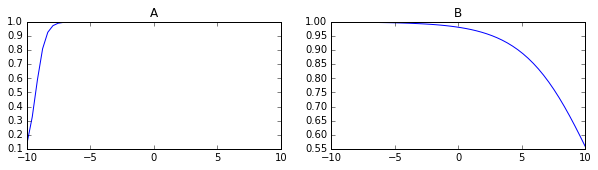
\includegraphics[width=\textwidth]{set1}
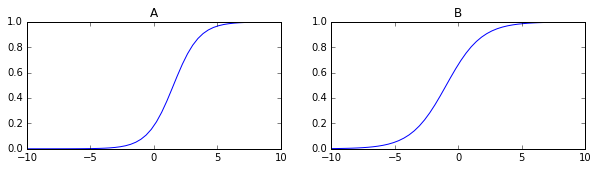
\includegraphics[width=\textwidth]{set2}
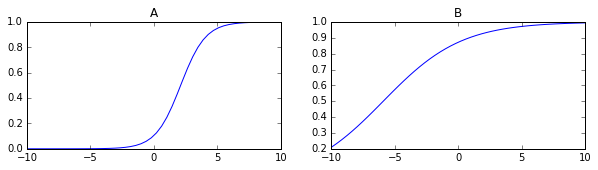
\includegraphics[width=\textwidth]{set3}
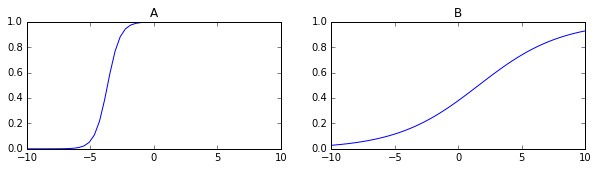
\includegraphics[width=\textwidth]{set4}
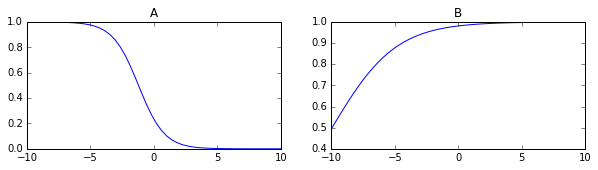
\includegraphics[width=\textwidth]{set5}
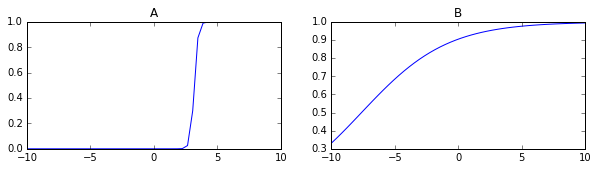
\includegraphics[width=\textwidth]{set6}
\section*{Analiza pogresaka}
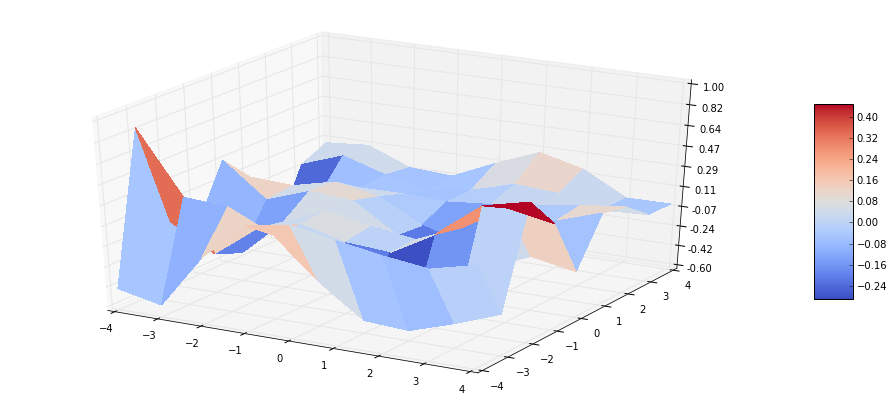
\includegraphics[width=\textwidth]{diff}
\section*{Usporedba batch i stochastic metoda}
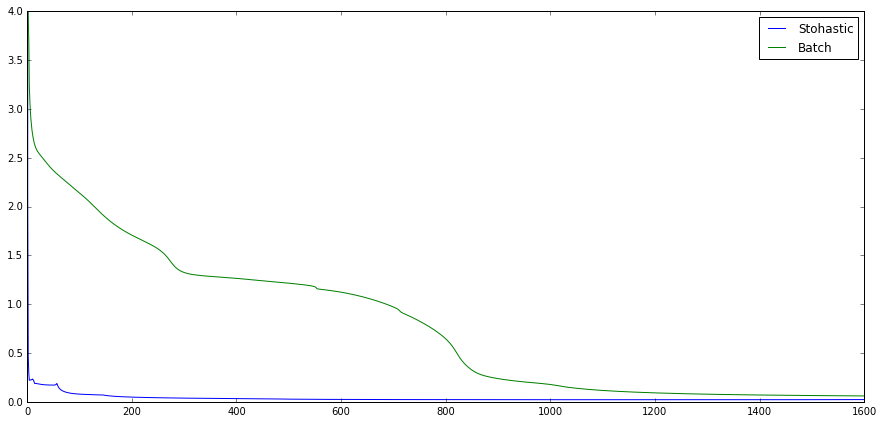
\includegraphics[width=\textwidth]{cmp1}
\section*{Usporedba stochastic metoda}
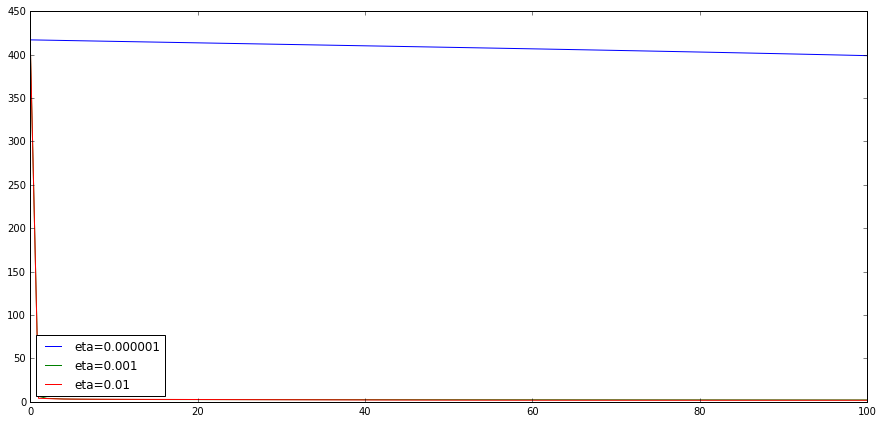
\includegraphics[width=\textwidth]{cmp2}
\section*{Usporedba batch metoda}
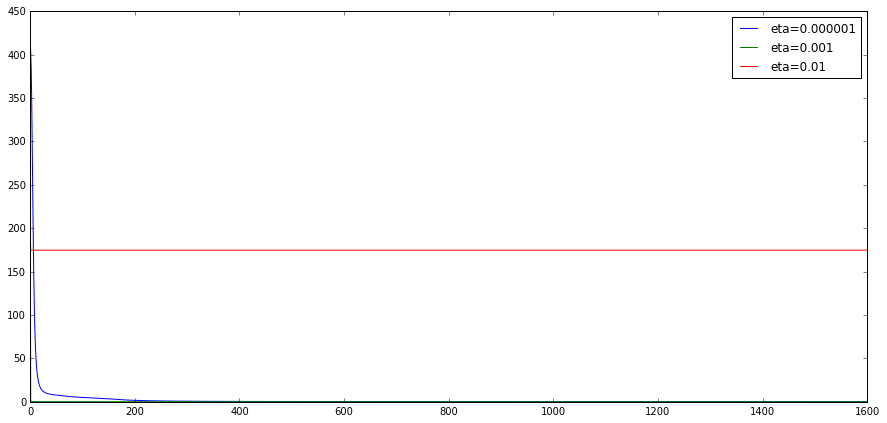
\includegraphics[width=\textwidth]{cmp3}


\end{document}
